From the wide set of examples of how the light can interact with matter in principle, the generalisation can be provided to create a distinction of three groups - reflection, propagation and transmittance. During its propagation in the body, the light can be:

\begin{itemize}
\item Refracted - bends of the light ray when inside the medium which cause the macroscopic effect in changing the light velocity when compared to the open space. 
\item Absorbed - as has been said before, it occurs when we have the resonant frequency of the light to provide a transition of a particle to the higher possible energy level. 
\item Emitted with luminescence process- is connected to the spontaneous emission but is not always provided after an absorption. The light emitted from the medium is in all directions and has different frequency than incident light(this is called the Stokes shift and will be explained later), if the absorption is its former inductor. 
\item Scattered - this changes the direction and sometimes the frequency of the input light. This is caused by the tiny changes of the frequency at the wavelength length scale. If the scale of the scattering centres are significantly smaller than the wavelength then we have the situation of the \textbf{Rayleigh scattering}.
\end{itemize}

It is also worth to note the refractive index of the medium as the change ratio of velocity in free space to velocity in the medium $n = \frac{c}{v}$. Its dispersion relation(connection to the frequency of the light) is directly connected to the inner processes that will be stated later on. 

Absorption inside the medium is also macroscopically described by the \textbf{Beer's law}. It creates a description as fraction of power that is absorbed by the unit length of the sample and has its exponential form of:

\begin{equation}
I(z) = I_0 e^{-\alpha z}
\end{equation}

where light propagates in the z direction, $I_0$ is intensity of the light at z = 0 and $\alpha$ is the absorption coefficient(which also has the dispersion relation). This can be even extended when generalise to the complex refractive index. 

\begin{equation}
\tilde{n} = n + i\kappa
\end{equation}

where n is the normal refractive index and $\kappa$ is an extinction coefficient and is directly connected to the $\alpha$ coefficient. Generalization of the wave vector $\mathbf{k}$ is 

\begin{equation}
k = \tilde{n} \frac{\omega}{c}
\end{equation}

so with the Beer's law we have that electric field is(because $I \propto$ square root of the electric field module):

\begin{equation}
\varepsilon (z,t) = \varepsilon _0 e^{\kappa \omega z/c} e^{i(\omega nz/c - \omega t)}
\end{equation}

So extinction coefficient isn't connected to the phase but to the exponential decay. We usually provide \textbf{complex relative dielectric constant} $\varepsilon _r$

\subsection{Interband absorption}
The fact that the semiconductors have the fundamental band gap creates a hard absorption edge in the spectra. The excitation between bands provide transitions for the certain range and leads to different processes later. The classical model of oscillatory electronic vibrations fails to deal with the discrete states as they are in the media, therefore we need to apply some quantum mechanics to provide the reliable description as we are dealing with nanostructures. As we said before, the difference between bands is the band gap $E_g$. Transitions between them are only possible when selection rules allow them and the frequency is fitted to it. If the there is electron possible to be excited we also need to fulfil the \textbf{Pauli exclusion principle} that states that the higher state must be empty. Let's say that the initial energy is $E_i$ and the electron is excited with a photon to the final energy $E_f$ above the band gap. This creates an electron-hole pair. 

\begin{equation}
Ef=Ei + h\omega
\end{equation} 

The band gap in semiconductors can be \textit{direct} or \textit{indirect}. The first case is when the maximum of the valence band and minimum of the conduction band is for the wavenumber k = 0. The second case is when conduction band minimum is moved at the different k. The transition rate from the initial state to the final state is provided by the \textbf{Fermi's Golden Rule}:


\begin{equation}
W_{i\rightarrow f} = \frac{2\pi}{\hbar}|M|^2g(\hbar \omega)
\end{equation}

where M is the transition matrix element and $g(\hbar \omega)$ is again the density of states. The first one is just the element of the Hamiltonian. 

\begin{equation}
M = \langle f|H'| i \rangle = \int \psi_f^* (\mathbf{r})H'(\mathbf{r})\psi_i(\mathbf{r}) d^3r
\end{equation}

of course, H' is not the standard Hamiltonian but the external perturbation inducted one and is connected to the incident light wave. With semiclassical model, where we don't quantize the electromagnetic wave but just electrons we have( using the electron \textbf{dipole moment} \textbf{d}):

\begin{equation}
H' =- \mathbf{d} \cdot \mathbf{\varepsilon} _{photon}
\end{equation}

where

\begin{equation}
\mathbf{\varepsilon} _{photon} (\mathbf{r}) = \mathbf{\varepsilon} _0 e^{\pm i \mathbf{k \cdot r}}
\end{equation}

To finish the calculation it is important to input the wavefunction of an electron but we will just state  the conservation of momentum as the Bloch theorem works only for crystalline solids. It is crucial that the change of electron momentum must be equal to the photon momentum so:

\begin{equation}
\hbar \mathbf{k_f} - \hbar \mathbf{k_i} = \pm \hbar \mathbf{k}
\end{equation}

For the indirect band materials, to conserve the momentum, we need to add emission or absorption of a phonon,  which changes the light absorption dependence. 

\subsection{Excitons}
Leaving the electron-hole pair in different bands provides a possibility of the mutual Coulomb interaction between them. This is an attractive interaction which possesses a very unique properties. 

Exciton can be considered as a small hydrogen like system. Two basic types of them are observed:

\begin{itemize}
\item Wannier-Mott excitons - free excitons
\item Frenkel excitons - tightly bound excitons
\end{itemize}

For their size, the Frenkel excitons are more probable to be found in molecular materials and nanostructures. 

\begin{figure}[H]
\centering
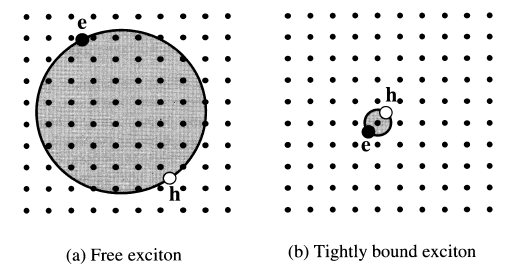
\includegraphics[width = 0.6\textwidth]{ch2/exciton}
\caption{Image that shows the characteristic difference between two types of excitons. Wannier-Mott excitons are not constrained to any atom and can move freely through the material in contrast to the Frenkel excitons which are much less mobile\cite{fox}}
\end{figure}

Stability of the exciton is strictly induced with the possibility of their potential to be big enough not to allow collisions with phonons.

\subsection{Photoluminescence}

Photoluminescence may be described as an emitted electromagnetic radiation as a result of its former excitation. The excited state depends on the internal energy structure of a radiated object and is an unique example of non equilibrium state. We might say from now on that during the whole luminescence process three possible scenarios are here to be observed. 
\begin{itemize}
\item Firstly the electron-hole pair is created.
\item The recombination process occurs.
\item Then the radiation escapes from our sample.
\end{itemize}

\begin{figure}[H]
\centering
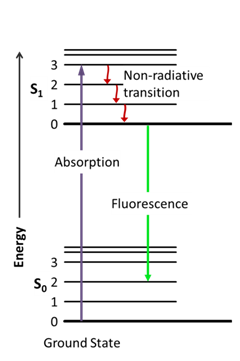
\includegraphics[height = 0.2\paperheight]{ch2/fluorescencediagram}
\caption{Example of few of the processes that are present during photoluminescence\cite{princeton}}
\end{figure}


The recombination is most probable near the surface of the sample, therefore the depletion of the carries is possible starting with the recombination processes with can be both radiative or non-radiative. Following that the recombination radiation is most usually emitted near the surface again, the great amount of experiments are created in the manner to directly look into the irradiated side.

The thing that luminescence can be accompanied to the absorption doesn't change the fact that it is quite different than it. In luminescence atoms emit light via the spontaneous emission so it's indivisibly defined by all of the vast majority of relaxation processes. The luminescence is divided into photoluminescence and electroluminescence. We can use it to study the bang gaps, transitions from it or transitions from deep doping states and defects. From the PL we can extract such informations as types and concentration of doping. Then, as we change the sample temperature we can also see how many relaxing centres are realised inside the medium. The possible relaxation types for exciton are shown in [Figure \ref{fig:relax}]
\begin{figure}[H]
\centering
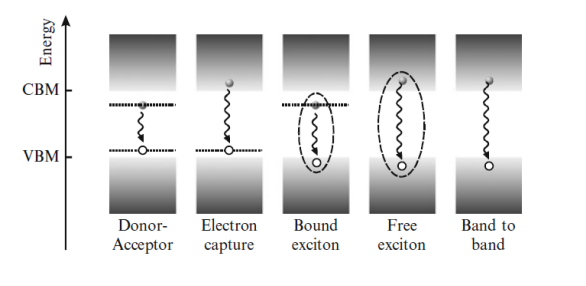
\includegraphics[width=0.5\textwidth]{ch2/recom}
\caption{Relaxation processes for excitons in the medium\cite{popko}}
\label{fig:relax}
\end{figure}

To describe spontaneous emission we can use Einstein A coefficient which is directly connected with B coefficient responsible for absorption and is different for different materials. When we have upper level populated at N at a time t we can say that:
\begin{equation}
\left( \frac{dN}{dt} \right) = -AN
\end{equation}
This tells us that emission behaves exponentially with $\tau_R $ being the radiative lifetime of a transition. The relaxation not always goes with photon emission, there can be a non-radiative one as well(f.e. as heat by creating lattice vibrations called phonons) and this is restricted by comparing the time-scales of emissions.  

\subsection{Quantum Confinement}

The properties of small systems are obviously rather different than those of bulk. The confinement in those kind of structures plays a crucial role in describing the physical properties. The first idea to describe semiconductors using quantum confinement and quantum mechanics methods has been used by Esaki and Tsu in 1970 \cite{Esaki1970}, which has lead to extreme advancement in describing the phenomena semiconductor physics. All thinks that are connected to optical properties of confined structures all directly derived from all the things that are connected to optical properties of solids described above. 

Changing the size of the crystal leads to great difference in the optical properties. The confinement effect in tiny regime leads us to the \textbf{Heisenberg uncertainty principle}, which tells us that the more we know the position of an object $\Delta x$, the less we know its momentum $\Delta p_x$

\begin{equation}
\Delta x \Delta p_x \geq \frac{\hbar}{4}
\end{equation}

This confinement leads to additional term to kinetic energy of particle with mass m connected to the uncertainty of momentum:

\begin{equation}
E_{con} = \frac{(\Delta p_x)^2}{2m}
\end{equation}

This energy can play an important part in its energy when it's comparable or greater than the thermal kinetic energy, which, let's say, on average is $\frac{1}{2}k_BT$.
This tells us that quantum effect will be considerable if the determined position is the size of $\sqrt{\frac{\hbar ^2}{mk_bT}}$. This can be transformed and stated that the position must be in the order of the \textbf{de Broglie} wavelength of an object $\lambda_{dB} \equiv \frac{p_x}{h}$.

Quantum confined structures are classified by the dimensions they are confined in.

\begin{itemize}
\item Quantum wells(confinement in 1-D)
\item Quantum wires(confinement in 2-D)
\item \textbf{Quantum dots}(confinement in 3-D)
\end{itemize}

The confinement of carriers in quantum dots describes that the carriers are completely localised on the particle. To describe the three dimensional confinement the model of the particle in a box has been used as a first method to the problem. Later on, it has been extended with more terms in the Hamiltonian like Coulomb interaction or non-parabolic and more complicated band structures. Those models have given rise to new properties such as: selection rules, radial wavefunction shape and the energy structures. This has shown that to truly understand the phenomena, we need to use non-linear optics as well. The beginning consists of going through one electron-hole pair(1EHP) states and then increasing the population and density of excited states by f.e differing the size of the nanoparticle. We will now state the 1EHP theory and tell where can it can be further explained. 

\begin{figure}
\centering
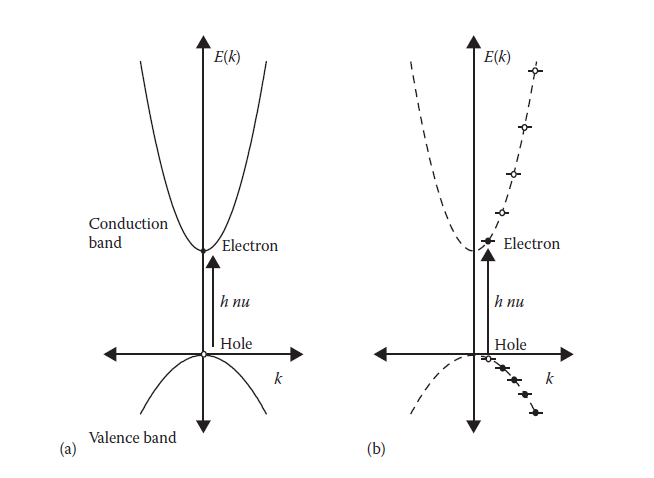
\includegraphics[width=0.65\textwidth]{ch2/energies}
\caption{The image of a band structure for two band model in direct band semiconductors a). In b) we can see that there are much more discrete states in a nanoparticle than in bulk a) \cite{Klimov}}
\end{figure}


\subsubsection{The Particle in a box}

This model is used in describing a behaviour of a particle with mass \textit{m} in a spherical potential with radius \textit{a}. \cite{Klimov} 

\[ V(r) = 
 \begin{cases}
 0  & r < a \\
 \infty & r \geq a
 \end{cases}
\]

where the radius can differ for holes and electron. This type of potential is connected with solving the stationary Schroedinger equation:

\begin{equation}
\hat{H}\Psi (\mathbf{r}) =  E\Psi (\mathbf{r})
\end{equation}

The potential containing the semiconductor sphere is relatively infinitely high. In that kind of environment, the wavefunction is a product of a Bloch function and a new envelope function. The periodic Bloch part shall be the same in the barrier and the well. 

\begin{equation}
u_k(r)_{barrier} = u_k(r)_well = u_k(r)
\end{equation}

The whole function now:

\begin{equation}
\Psi (r) = \psi (r) u_k(r)
\end{equation}

where $\psi(r)$ is the new envelope function for electrons and holes. We now have that(neglecting the other interactions - in single parabolic band approximation):

\begin{equation}
\hat{H} = \left[ \frac{-\hbar ^2}{2m_e}\nabla _e^2 \frac{-\hbar ^2}{2m_h}\nabla _h^2 \right] + V_e(\mathbf{r}) + V_h(\mathbf{r}) =
\end{equation}

The envelope function is separable for holes and electrons so the solutions have a shape like:

\begin{equation}
\Phi _{nlm} ^i(r) = Y_{lm} \sqrt{\frac{2}{R^3}} \frac{J_l(\chi _{nl}\frac{r}{R}}{J_{l+1}(\chi _{nl})}
\end{equation}

where $-l \leq m \leq l; l = 0,1,2,3...; n = 1,2,3,...$, $Y_{lm}$ are spherical harmonics and $J_l$ are the Bessel functions and $\chi _{nl}$ is the n-th zero of order l Bessel function. When we put effective masses we can estimate roots and calculate the energy levels for the envelope functions. Then we can calculate the optical properties calculating the overlap of the functions. Nevertheless, this approximation cannot fully explain what happens with the nanoparticles, we have simply neglected all the things that are making them different like Bloch functions, interactions etc. The next step would be to add interactions, mixing, splitting and then process to the other states as has been said at the beginning. This is rather Complex method, and the first thing you can do is to use the so called $k\cdot p$ perturbation theory to approximate some of the things and make calculations easier. As it is not the topic of the thesis, the places where you can read it further are here \cite{Klimov} \cite{ulrike} \cite{fox} \cite{dotsy}